\documentclass[tikz,border=6pt]{standalone}
\usepackage{tikz}
\usetikzlibrary{arrows.meta}
\definecolor{nebula}{HTML}{6366F1}
\definecolor{spark}{HTML}{14B8A6}
\definecolor{ink}{HTML}{334155}
\begin{document}
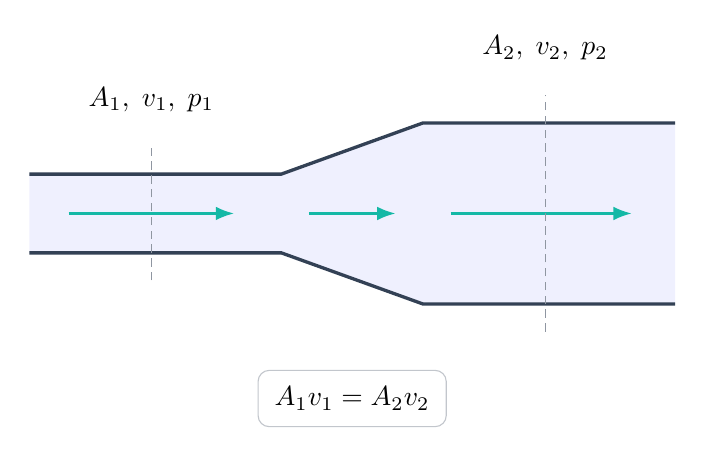
\begin{tikzpicture}[font=\sffamily,>=Latex]
  \fill[nebula!10] (0,2.5)--(3.2,2.5)--(5,3.15)--(8.2,3.15)--(8.2,.85)--(5,.85)--(3.2,1.5)--(0,1.5)--cycle;
  \draw[very thick,ink] (0,2.5)--(3.2,2.5)--(5,3.15)--(8.2,3.15);
  \draw[very thick,ink] (0,1.5)--(3.2,1.5)--(5,.85)--(8.2,.85);
  \draw[->,thick,spark] (.5,2)--(2.6,2);
  \draw[->,thick,spark] (3.55,2)--(4.65,2);
  \draw[->,thick,spark] (5.35,2)--(7.65,2);
  \draw[densely dashed,ink!55] (1.55,1.15)--(1.55,2.85);
  \draw[densely dashed,ink!55] (6.55,.5)--(6.55,3.5);
  \node[align=center,fill=white,inner sep=3pt] at (1.55,3.45) {$A_1,\;v_1,\;p_1$};
  \node[align=center,fill=white,inner sep=3pt] at (6.55,4.1) {$A_2,\;v_2,\;p_2$};
  \node[draw=ink!30,rounded corners=4pt,fill=white,inner sep=6pt] at (4.1,-.35) {$A_1v_1=A_2v_2$};
\end{tikzpicture}
\end{document}
